\subsection{Are over-parametrized networks undoing what the previous layers have done?}
\label{sec:overparametrized_undoing}

\Cref{sec:weight_tied} showed that one shared stage-3 block nearly matches nine
independent ones ($-0.61$ top-1 points, $33\%$ fewer parameters).
A natural explanation is that the untied stack is over-parametrised along depth:
consecutive blocks need not push the state in a coherent direction, and part of
what block $k{+}1$ does can cancel what block $k$ just did.
We test that claim directly on feature trajectories, using the same 500 ImageNet
validation images (one per class) as in \cref{sec:geometrical_analysis}, stage~3
only, with the massive channel removed (\cref{sec:massive_activations}).

\paragraph{Setup.}
For each image we integrate the stage from $t{=}0$ to $t{=}9$ at native resolution
($R{=}1$) and under Euler refinement ($R{=}100$, $\Delta t{=}0.01$), and reduce every
spatial feature coordinate whose net displacement $|\Delta_i|=|x_i(9)-x_i(0)|$ is above
the per-image median.
We partition the trajectory into the nine unit intervals $[k,k{+}1]$ (native blocks
in ConvNeXt-T; the same time bins in the weight-tied model) and write
$\mathrm{d}x_k$ for the displacement of a coordinate over interval $k$.
The scalars we report are means $\pm$ std over the 500 images
(\cref{tab:undo}):
\begin{itemize}
    \item \emph{straightness}: $\|\sum_k\mathrm{d}x_k\|\,/\,\sum_k\|\mathrm{d}x_k\|$
    in feature space (path length vs.\ net displacement);
    \item \emph{wasted motion}: $1-\sum_i|\mathrm{net}_i|/\sum_{k,i}|\mathrm{d}x_{k,i}|$,
    the fraction of per-coordinate travel that cancels before $t{=}9$;
    \item $\cos(\mathrm{d}x_k,\mathrm{d}x_{k+1})$: mean cosine between consecutive
    block displacements;
    \item \emph{undo fraction}: when $\mathrm{sign}(\mathrm{d}x_k)$ flips at the next
    block, the cancelled mass
    $\min(|\mathrm{d}x_k|,|\mathrm{d}x_{k+1}|)$ normalised by $\sum|\mathrm{d}x_k|$;
    \item \emph{zig-zag share}: mass-weighted share of coordinates that reverse at
    least twice across the nine blocks;
    \item \emph{sign flips at $t\in\mathbb{N}$}: fraction of consecutive steps whose
    sign changes exactly at integer depths (block boundaries).
\end{itemize}

\begin{table*}[t]
    \centering
    \caption{Pooled stage-3 trajectory statistics over 500 ImageNet images
    (massive channel ignored; coordinates with $|\Delta_i|$ above the per-image median).
    Weight-tied vs.\ standard ConvNeXt-T at native ($R{=}1$) and refined ($R{=}100$)
    resolution. Mean $\pm$ std across images.}
    \label{tab:undo}
    \scriptsize
    \setlength{\tabcolsep}{3.5pt}
    \resizebox{\textwidth}{!}{%
    \begin{tabular}{llccccccccc}
\toprule
Model & $R$ & straightness & wasted motion & monotone share & $\cos(\Delta x_k,\Delta x_{k+1})$ & reversal rate & undo fraction & zig-zag share & sign flips at $t\in\mathbb{N}$ & median $t_{50}$ \\
\midrule
Weight-tied ConvNeXt & 100 & 0.78$\pm$0.02 & 0.19$\pm$0.01 & 0.73$\pm$0.02 & 0.92$\pm$0.01 & 0.11$\pm$0.01 & 0.02$\pm$0.00 & 0.14$\pm$0.02 & 0.00$\pm$0.00 & 4.09$\pm$0.16 \\
ConvNeXt-T & 100 & 0.50$\pm$0.01 & 0.48$\pm$0.01 & 0.21$\pm$0.01 & 0.17$\pm$0.01 & 0.45$\pm$0.00 & 0.25$\pm$0.00 & 0.90$\pm$0.00 & 0.45$\pm$0.00 & 7.21$\pm$0.15 \\
Weight-tied ConvNeXt & 1 & 0.72$\pm$0.02 & 0.25$\pm$0.02 & 0.63$\pm$0.03 & 0.77$\pm$0.03 & 0.18$\pm$0.01 & 0.05$\pm$0.01 & 0.34$\pm$0.03 & 0.18$\pm$0.01 & 5.00$\pm$0.09 \\
ConvNeXt-T & 1 & 0.50$\pm$0.01 & 0.48$\pm$0.01 & 0.22$\pm$0.01 & 0.16$\pm$0.01 & 0.45$\pm$0.00 & 0.25$\pm$0.00 & 0.90$\pm$0.00 & 0.45$\pm$0.00 & 7.82$\pm$0.38 \\
\bottomrule
\end{tabular}

    }
\end{table*}

\begin{figure*}[t]
    \centering
    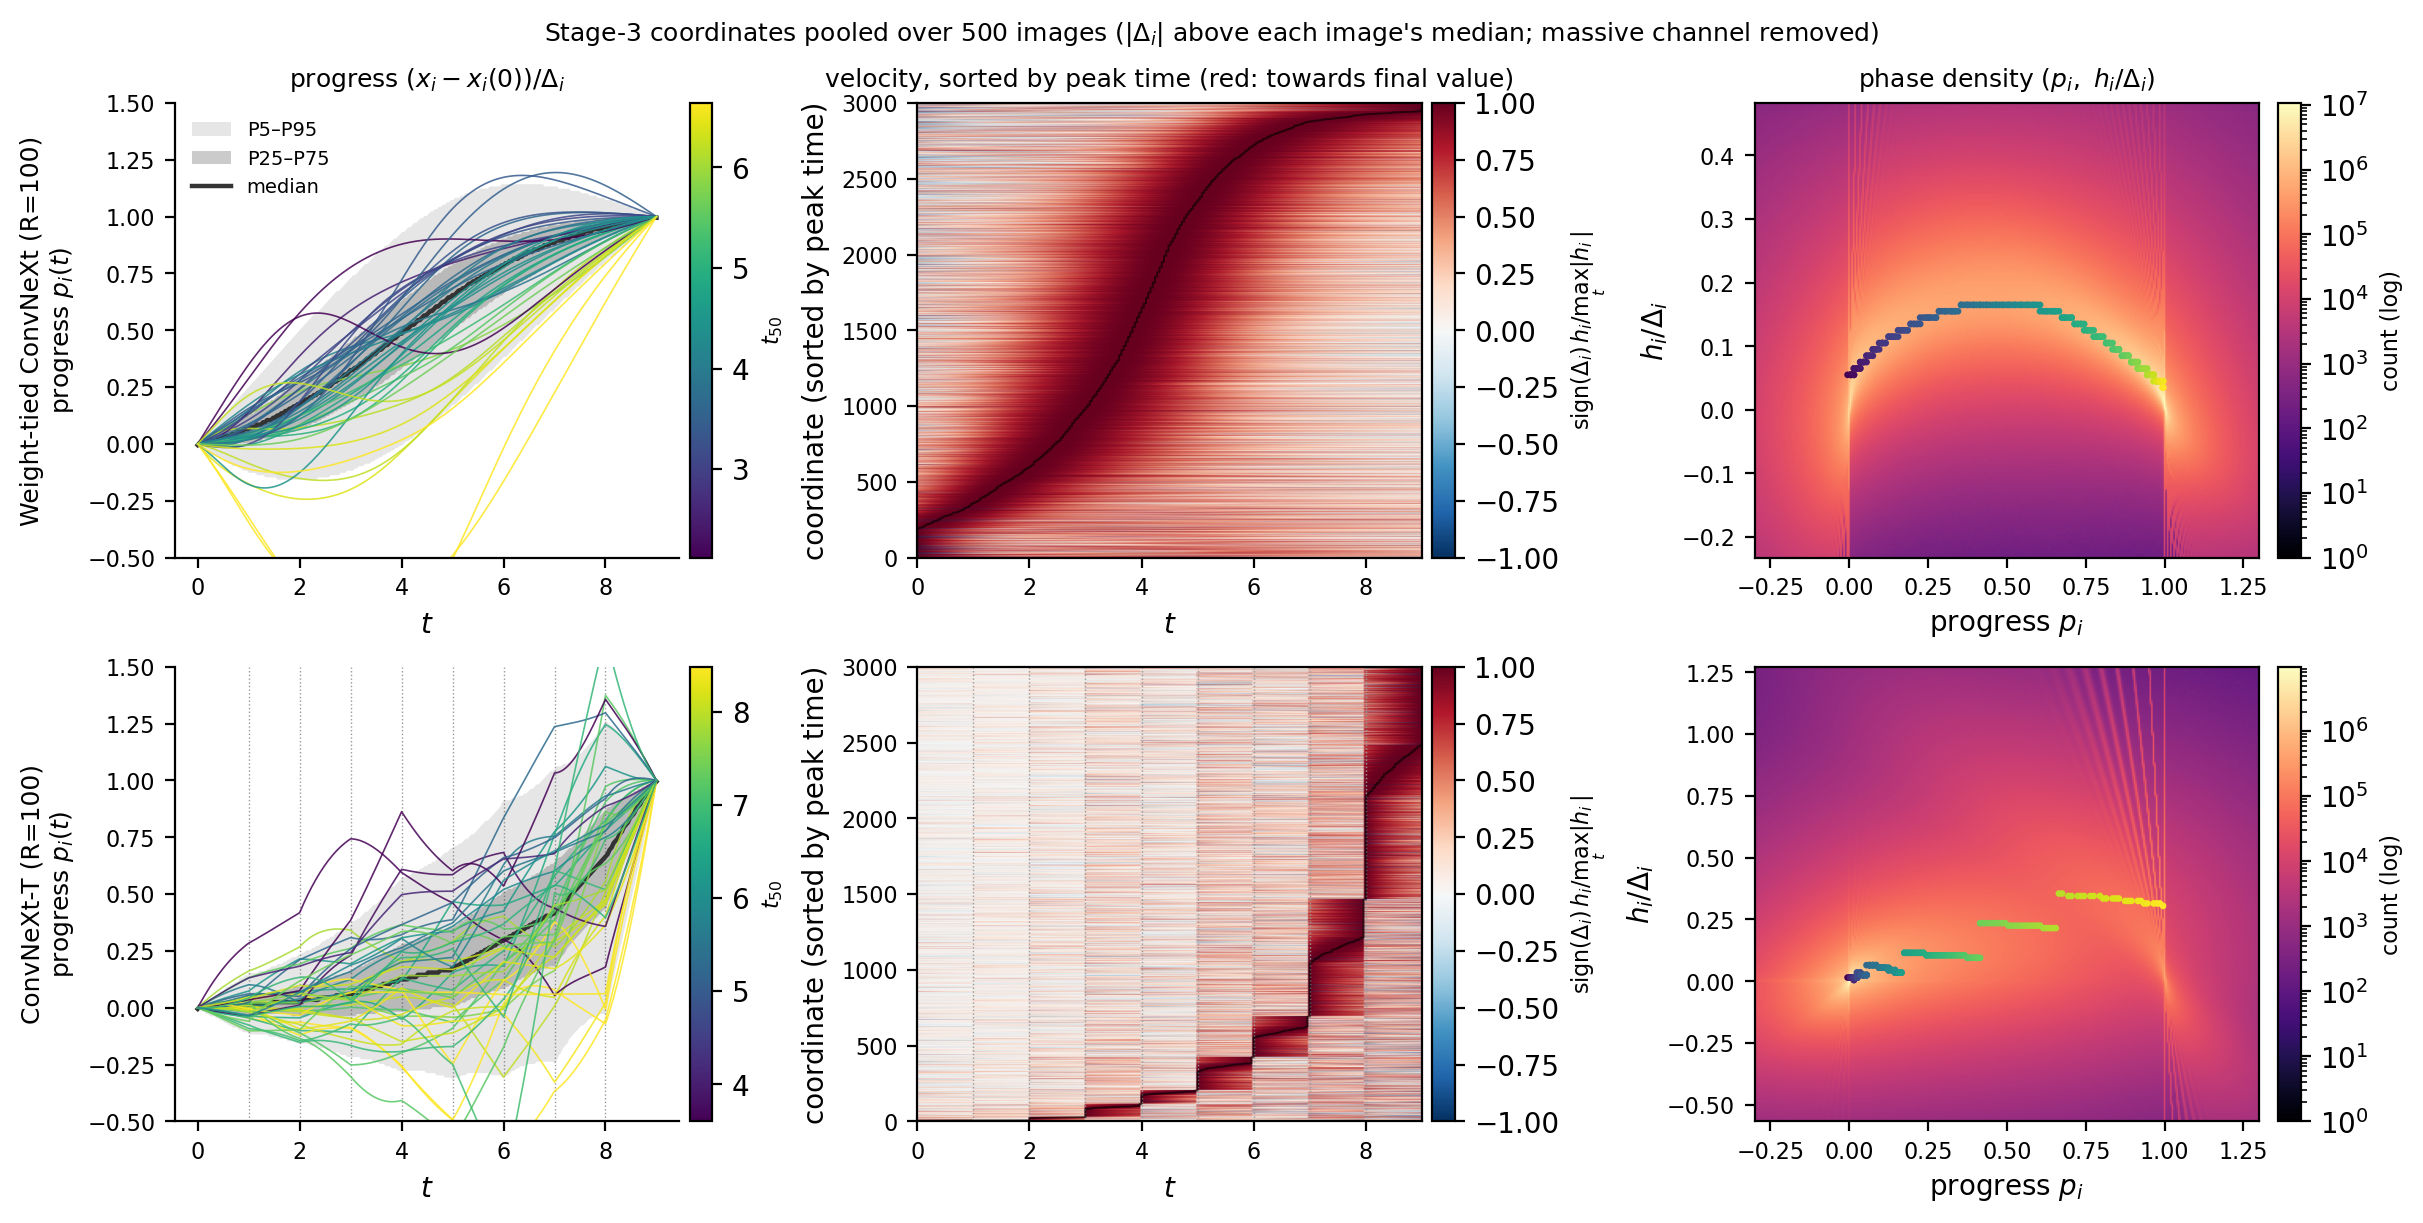
\includegraphics[width=\textwidth]{figures/pooled_dynamics.png}
    \caption{Stage-3 coordinates pooled over 500 images ($R{=}100$; massive channel
    removed; $|\Delta_i|$ above the per-image median).
    \textbf{Top:} weight-tied ConvNeXt; \textbf{bottom:} ConvNeXt-T.
    \textbf{Left:} progress $p_i(t)=(x_i(t)-x_i(0))/\Delta_i$ (median and P5--P95;
    thin lines: random coordinates).
    \textbf{Middle:} velocity toward the final value, coordinates sorted by peak time
    (red: toward the end state; blue: away).
    \textbf{Right:} phase density $(p_i,\,h_i/\Delta_i)$.
    The shared field advances mostly monotonically; the switched stack reverses and
    rewrites features between blocks.}
    \label{fig:pooled-dynamics}
\end{figure*}

\paragraph{Results.}
\Cref{tab:undo} and \cref{fig:pooled-dynamics} give a consistent picture.
Under refinement ($R{=}100$), the weight-tied model is nearly monotone along depth:
straightness $0.78$, wasted motion $0.19$, consecutive-block cosine $0.92$, undo
fraction $0.02$, and zig-zag share $0.14$.
Sign changes at integer times are essentially absent ($0.00$).
ConvNeXt-T, with nine independent blocks, sits at the opposite extreme: straightness
$0.50$, wasted motion $0.48$ (almost half of the travel cancels), cosine $0.17$,
undo fraction $0.25$ ($\approx 12\times$ the shared value), and zig-zag share $0.90$.
Nearly half of the sign flips ($0.45$) fall exactly on block boundaries---the
discontinuities of the switched field in \cref{sec:teaser-b}, not an artefact of a
coarse step.
Native resolution ($R{=}1$) barely changes the ConvNeXt-T numbers; refining only
makes the shared field look cleaner (undo $0.05\to 0.02$), which matches the bounded
refinement error of \cref{sec:refinement_error}.

\paragraph{Functional progress along depth.}
Geometry shows wasted motion; a complementary probe asks when the stage~3 state
becomes usable by the rest of the network.
For each $k{=}1,\ldots,9$ we stop after the $k$-th residual block and classify with
the model's own trained downsample, stage~4 and head---no remaining stage~3 blocks
(\cref{fig:prefix-acc}; full ImageNet validation).
Under weight tying the top-1 rises early and smoothly: $33.6\%$ after one block,
$72.2\%$ after three, and $78.9\%$ by block~5, already close to the final
$80.3\%$.
On standard ConvNeXt-T the same frozen decoder stays weak for longer
($11.5\%$, $33.2\%$, $66.9\%$ at those depths) and only approaches the final
$81.0\%$ in the last few blocks.
Mid-stage accuracy is not a claim that early features lack information---the head
was trained on $x_T$---but it does show that the tied path enters the decoder's
operating region steadily, whereas the untied path aligns with that region late,
consistent with a transport that rewrites features before committing.

\begin{figure}[t]
    \centering
    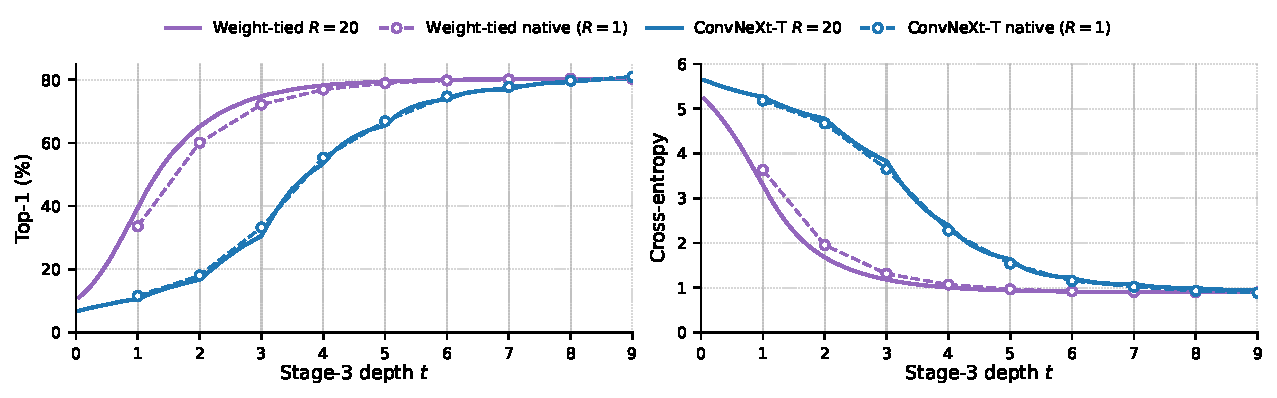
\includegraphics[width=0.7\linewidth]{figures/prefix_s4_head_acc.pdf}
    \caption{ImageNet top-1 of each model's trained stage~4+head on stage~3
    prefixes: after $k$ residual blocks, skip the rest of stage~3 and decode.
    Weight-tied features become usable earlier and more evenly; ConvNeXt-T
    concentrates most of the gain toward the end of the stage.}
    \label{fig:prefix-acc}
\end{figure}

\paragraph{Reading.}
Untied stage~3 does not implement nine steps of one transport: consecutive blocks
often point in weakly related or opposing directions and cancel a large fraction of
each other's work.
The weight-tied network cannot cancel itself in that way---a single autonomous field
has no ``next block'' with different weights---and the geometry shows almost no
undoing.
\Cref{fig:prefix-acc} makes the same contrast in function space: tied depth builds
decoder-ready features gradually, while untied depth postpones most of the usable
progress.
That is why sharing the nine blocks costs less than one top-1 point
(\cref{sec:weight_tied}): much of the untied capacity along depth is spent
rewriting features rather than accumulating a coherent displacement toward $x_T$.
The residual accuracy gap to the baseline is then more plausibly attributed to the
small, non-cancellable specialization that independent $\theta_k$ still provide, not to
a fundamentally different dynamical mechanism.
